\documentclass[../main/main.tex]{subfiles}
\begin{document}
\dominitoc
\faketableofcontents
\setcounter{chapter}{7}
\chapter{Validation du pipeline
  \hypergal}\label{ch:simu}

\minitoc
\vspace{2cm}
Nous avons présenté et détaillé dans le chapitre précédent le
fonctionnement du pipeline \hypergal. Après s'être assuré de sa
stabilité numérique, nous avons cherché une méthode de validation de son
efficacité. L'objectif est ainsi de quantifier la précision d'extraction
des spectres de supernovae en fonction des conditions d'observation, et
la capacité d'\hypergal\ à les classifier.
Nous avons pour cela choisi de procéder à des simulations de cube
d'observation avec la SEDm.

Dans ce chapitre nous présenterons dans un premier temps la procédure de
génération des simulations, puis nous présenterons les résultats ainsi
obtenus de
l'utilisation d'\hypergal\ sur ces cubes simulés. 
\newpage

\section{Génération des simulations}
%\label{sec:xxx}

\subsection{Méthode}

Afin de se rapprocher au plus près des conditions d'observation, nous
avons profité de quelques périodes de mise hors service de la caméra
principale ZTF (entre fin novembre 2021 et fin janvier 2022): nous avons ainsi
pu utiliser occasionnellement la SEDm pour observer des galaxies hôtes isolées, dans
lesquelles une supernova a été observée dans le passé.

Nos simulations sont ainsi basées sur une dizaine de ces cubes, extraits
avec l'instrument pour lequel nous souhaitons tester \hypergal, et
contenant dans le champ de vue une galaxie et un fond réels.

Le but est ainsi de rajouter une composante de supernova dans ces
cubes en marginalisant sur les conditions d'observation habituelles
comme le seeing, ou la proportion de chaque type de supernova, tout en explorant
les conditions influants sur la robustesse d'\hypergal\ comme la distance
entre la source ponctuelle et le centre galactique, et le rapport signal
sur bruit.

Pour notre étude nous avons créé un jeu de $5000$ cubes de simulations,
et nous  détaillons dans cette section leur conception.

\subsection{Cube de galaxies isolées}
%\label{ssec:xxx}

La base de nos simulations proviennent donc d'observations réelles avec
la SEDm de galaxies ayant accueilli au moins un an dans le passé une
supernova.
Ces cubes sont donc naturellement dans l'espace de l'instrument pour
lequel \hypergal\ a été conçu.

Les effets d'ADR sont également présents, et il faut donc bien les
caractériser avant d'inclure une composante de supernova pour que celle
ci soit soumise aux mêmes effets chromatiques. 
Bien que nous connaissons à priori la masse d'air et l'angle
parallactique au début de l'observation, nous ne connaissons pas ces
paramètres effectifs, car ils varient au cours de l'exposition
(de l'ordre d'une demi-heure de temps de pose).

Nous avons pour cela inclus dans \hypergal\ la flexibilité de prendre en
compte ou non n'importe laquelle des composantes de scène, et avons
procéder à l'ajustement de scène avec uniquement la galaxie hôte dans le
MLA. Tout comme détaillé au chapitre précédent, l'ajustement du
centroïde à chaque méta-tranche nous permet d'ajuster les paramètres
effectifs d'ADR. Nos cubes présentent dans notre simulation une masse
d'air allant de $1.01$ à $2.04$, ce qui nous permet de couvrir les
conditions idéales d'observations, les conditions habituelles et les
conditions dégradées.

Nous montrons dans la Figure~\ref{fig:allhostsimu} les cubes intégrés
des galaxies hôtes utilisés pour les simulations.
\begin{figure}[ht]
  \centering
  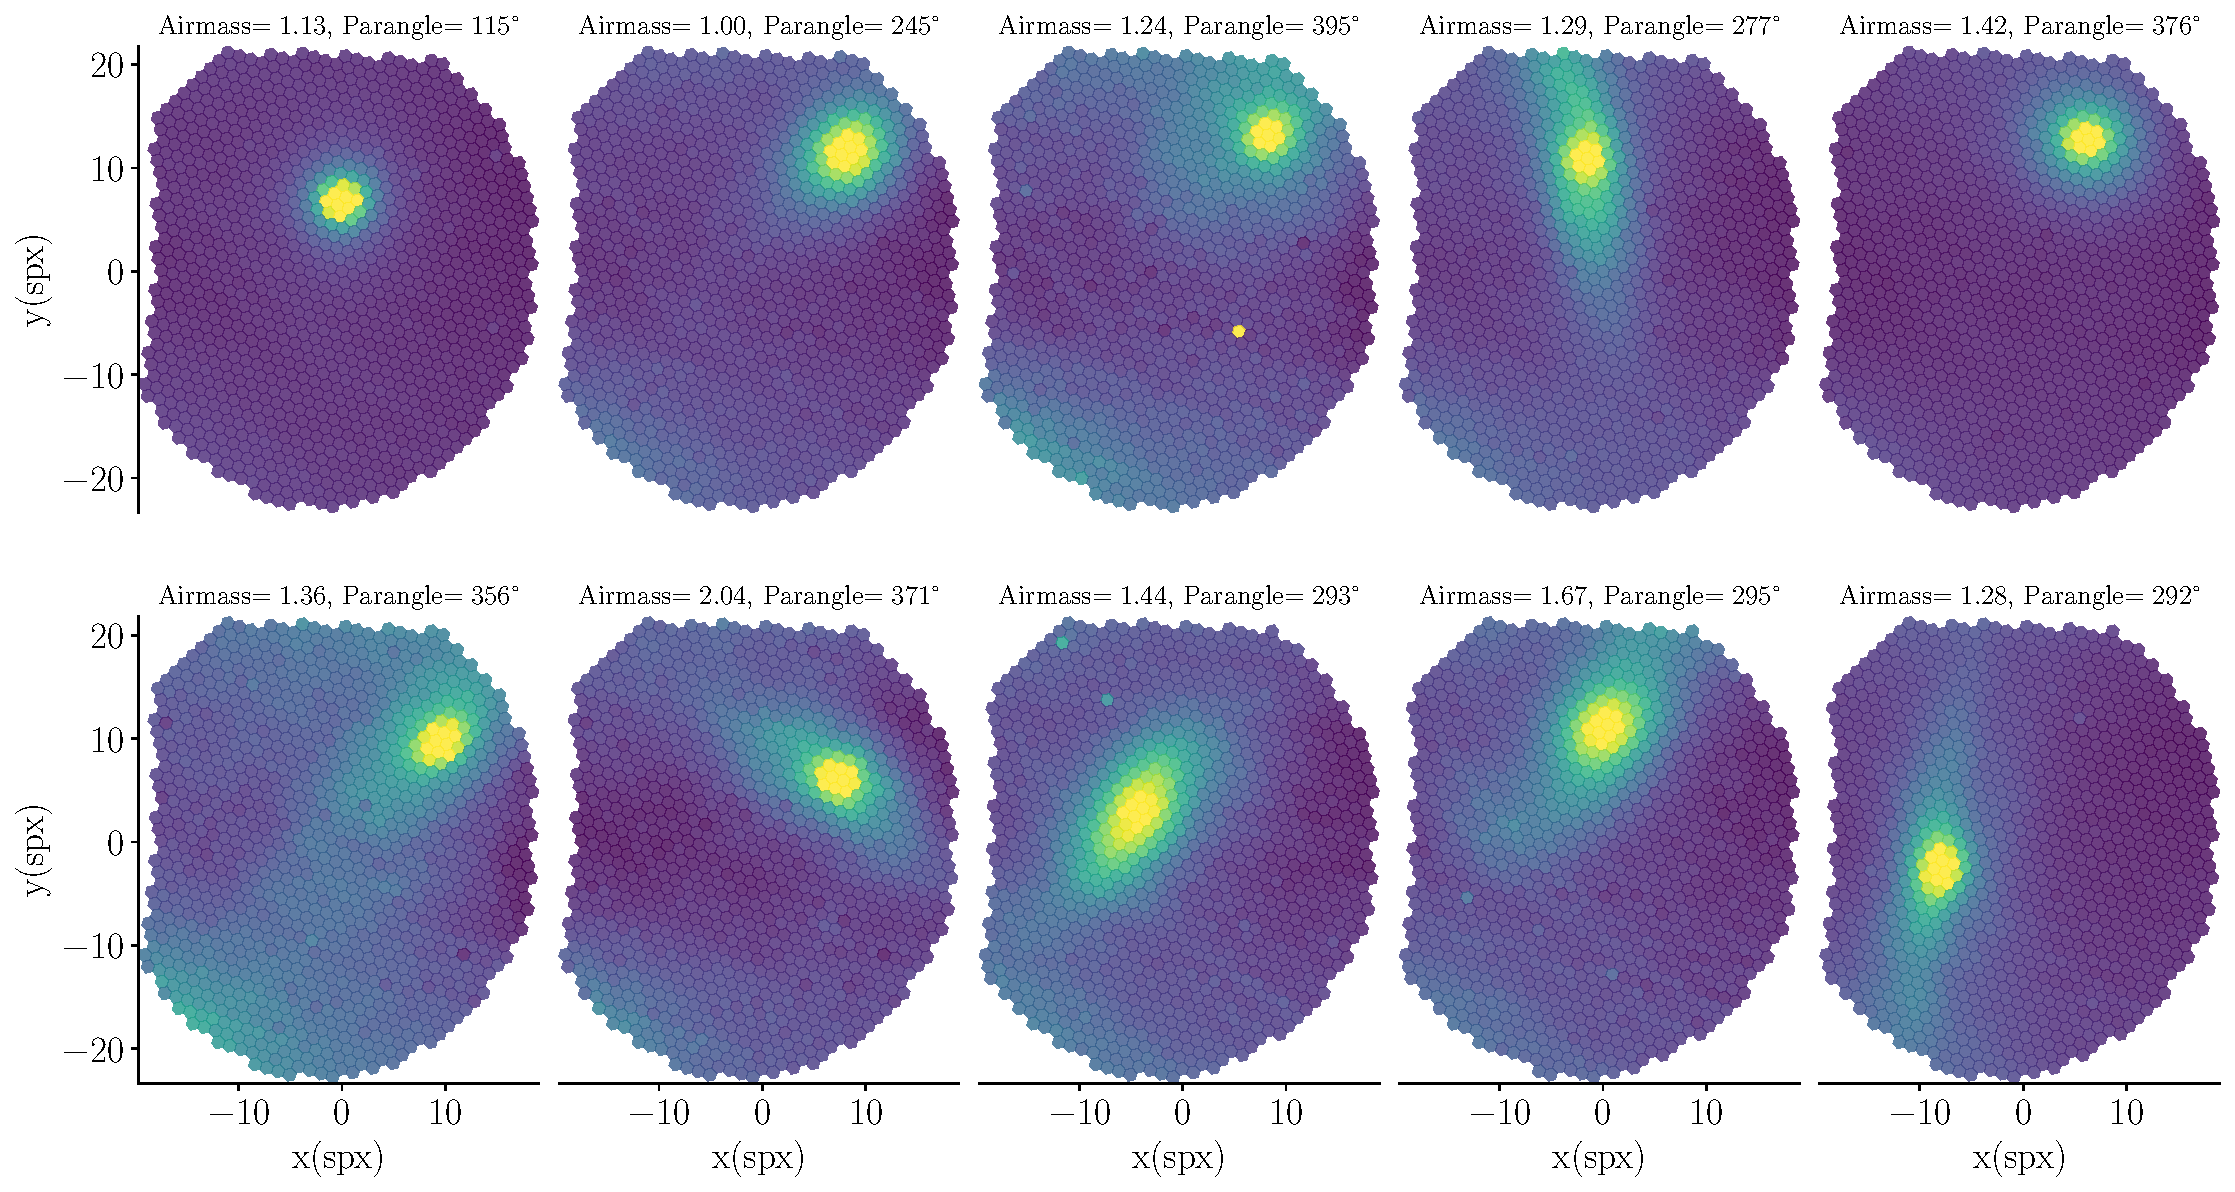
\includegraphics[width=0.99\textwidth]{../figures/08_simu/allhostsimu.pdf}
  \caption[Cubes de galaxies hôtes utilisés pour les simulations.]{Cubes
    intégrés des galaxies hôtes utilisés pour les simulations. Bien que
    nous n'ayons pas eu l'opportunité d'avoir un grand nombre
    d'observations de galaxies isolées avec la SEDm, nous avons fait
    l'hypothèse que ces morphologies et localisations variées de ces
    galaxies étaient suffisamment représentatives des observations pour
    constituer la base des simulations.}
  \label{fig:allhostsimu}
\end{figure}

\subsection{Modèles de supernovae}
% \label{ssec:xxx}

Afin de tester la précision d'extraction de spectre avec \hypergal, il nous faut inclure dans les cubes une source ponctuelle dont le
spectre est connu a priori. Cette étude est indépendante de la forme du spectre, et donc du type
de la supernova.
Cependant nous souhaitons également avoir une
estimation de l'efficacité d'\hypergal\ à classifier les supernovae.
Pour analyser ces deux aspects (précision et classification), il faut
donc que le spectre de la source ponctuelle simulée soit connu a priori et que nous connaissons sa classification.

Par manque de temps et pour éviter de devoir générer des spectres avec
des outils inconnus, puis les projeter dans l'espace des observations de
la SEDm (transmission, LSF, échantillonnage ...), nous avons choisi
d'utiliser des spectres de supernovae déjà obtenus avec la SEDm, et
classifiés avec SNID.

Afin de s'assurer de la classification, nous n'avons sélectionné que des
spectres avec un très haut r$lap$ (paramètre de qualité/confiance de SNID, considéré
comme bon si r$lap>5$). Pour les spectres de supernovae de type Ia (les plus nombreuses), nous avons
sélectionné $70$ spectres avec un r$lap>25$ pour le meilleur modèle, et un r$lap>15$ pour les 30 premiers modèles.

Sur un raisonnement similaire, nous avons sélectionné $7$ spectres de
supernova de type II avec un r$lap>12$. Pour les types Ic et Ib, plus
rarement observés ($\approx5\%$ des observations), nous avons préféré
prendre seulement $1$ spectre de chaque mais avec une très forte
confiance de classification ( r$lap\approx18$ pour la Ib et r$lap\approx15$
pour la Ic).

Nous procédons ensuite sur chacun de ces spectre à un lissage en
appliquant un filtre de Savitzky-Golay \citep{SavitzkyGolay}. Afin de ne pas casser les
structures des spectres, nous utilisons un lissage léger avec un
polynôme d'ordre 3 sur une fenêtre de 5 pixels.

Nous montrons dans la Figure~\ref{fig:specsimueach} un exemple de
spectre après lissage pour chaque type de supernova, ainsi que le
meilleur modèle de classification SNID et le r$lap$ associé.

\begin{figure}[ht]
  \centering
  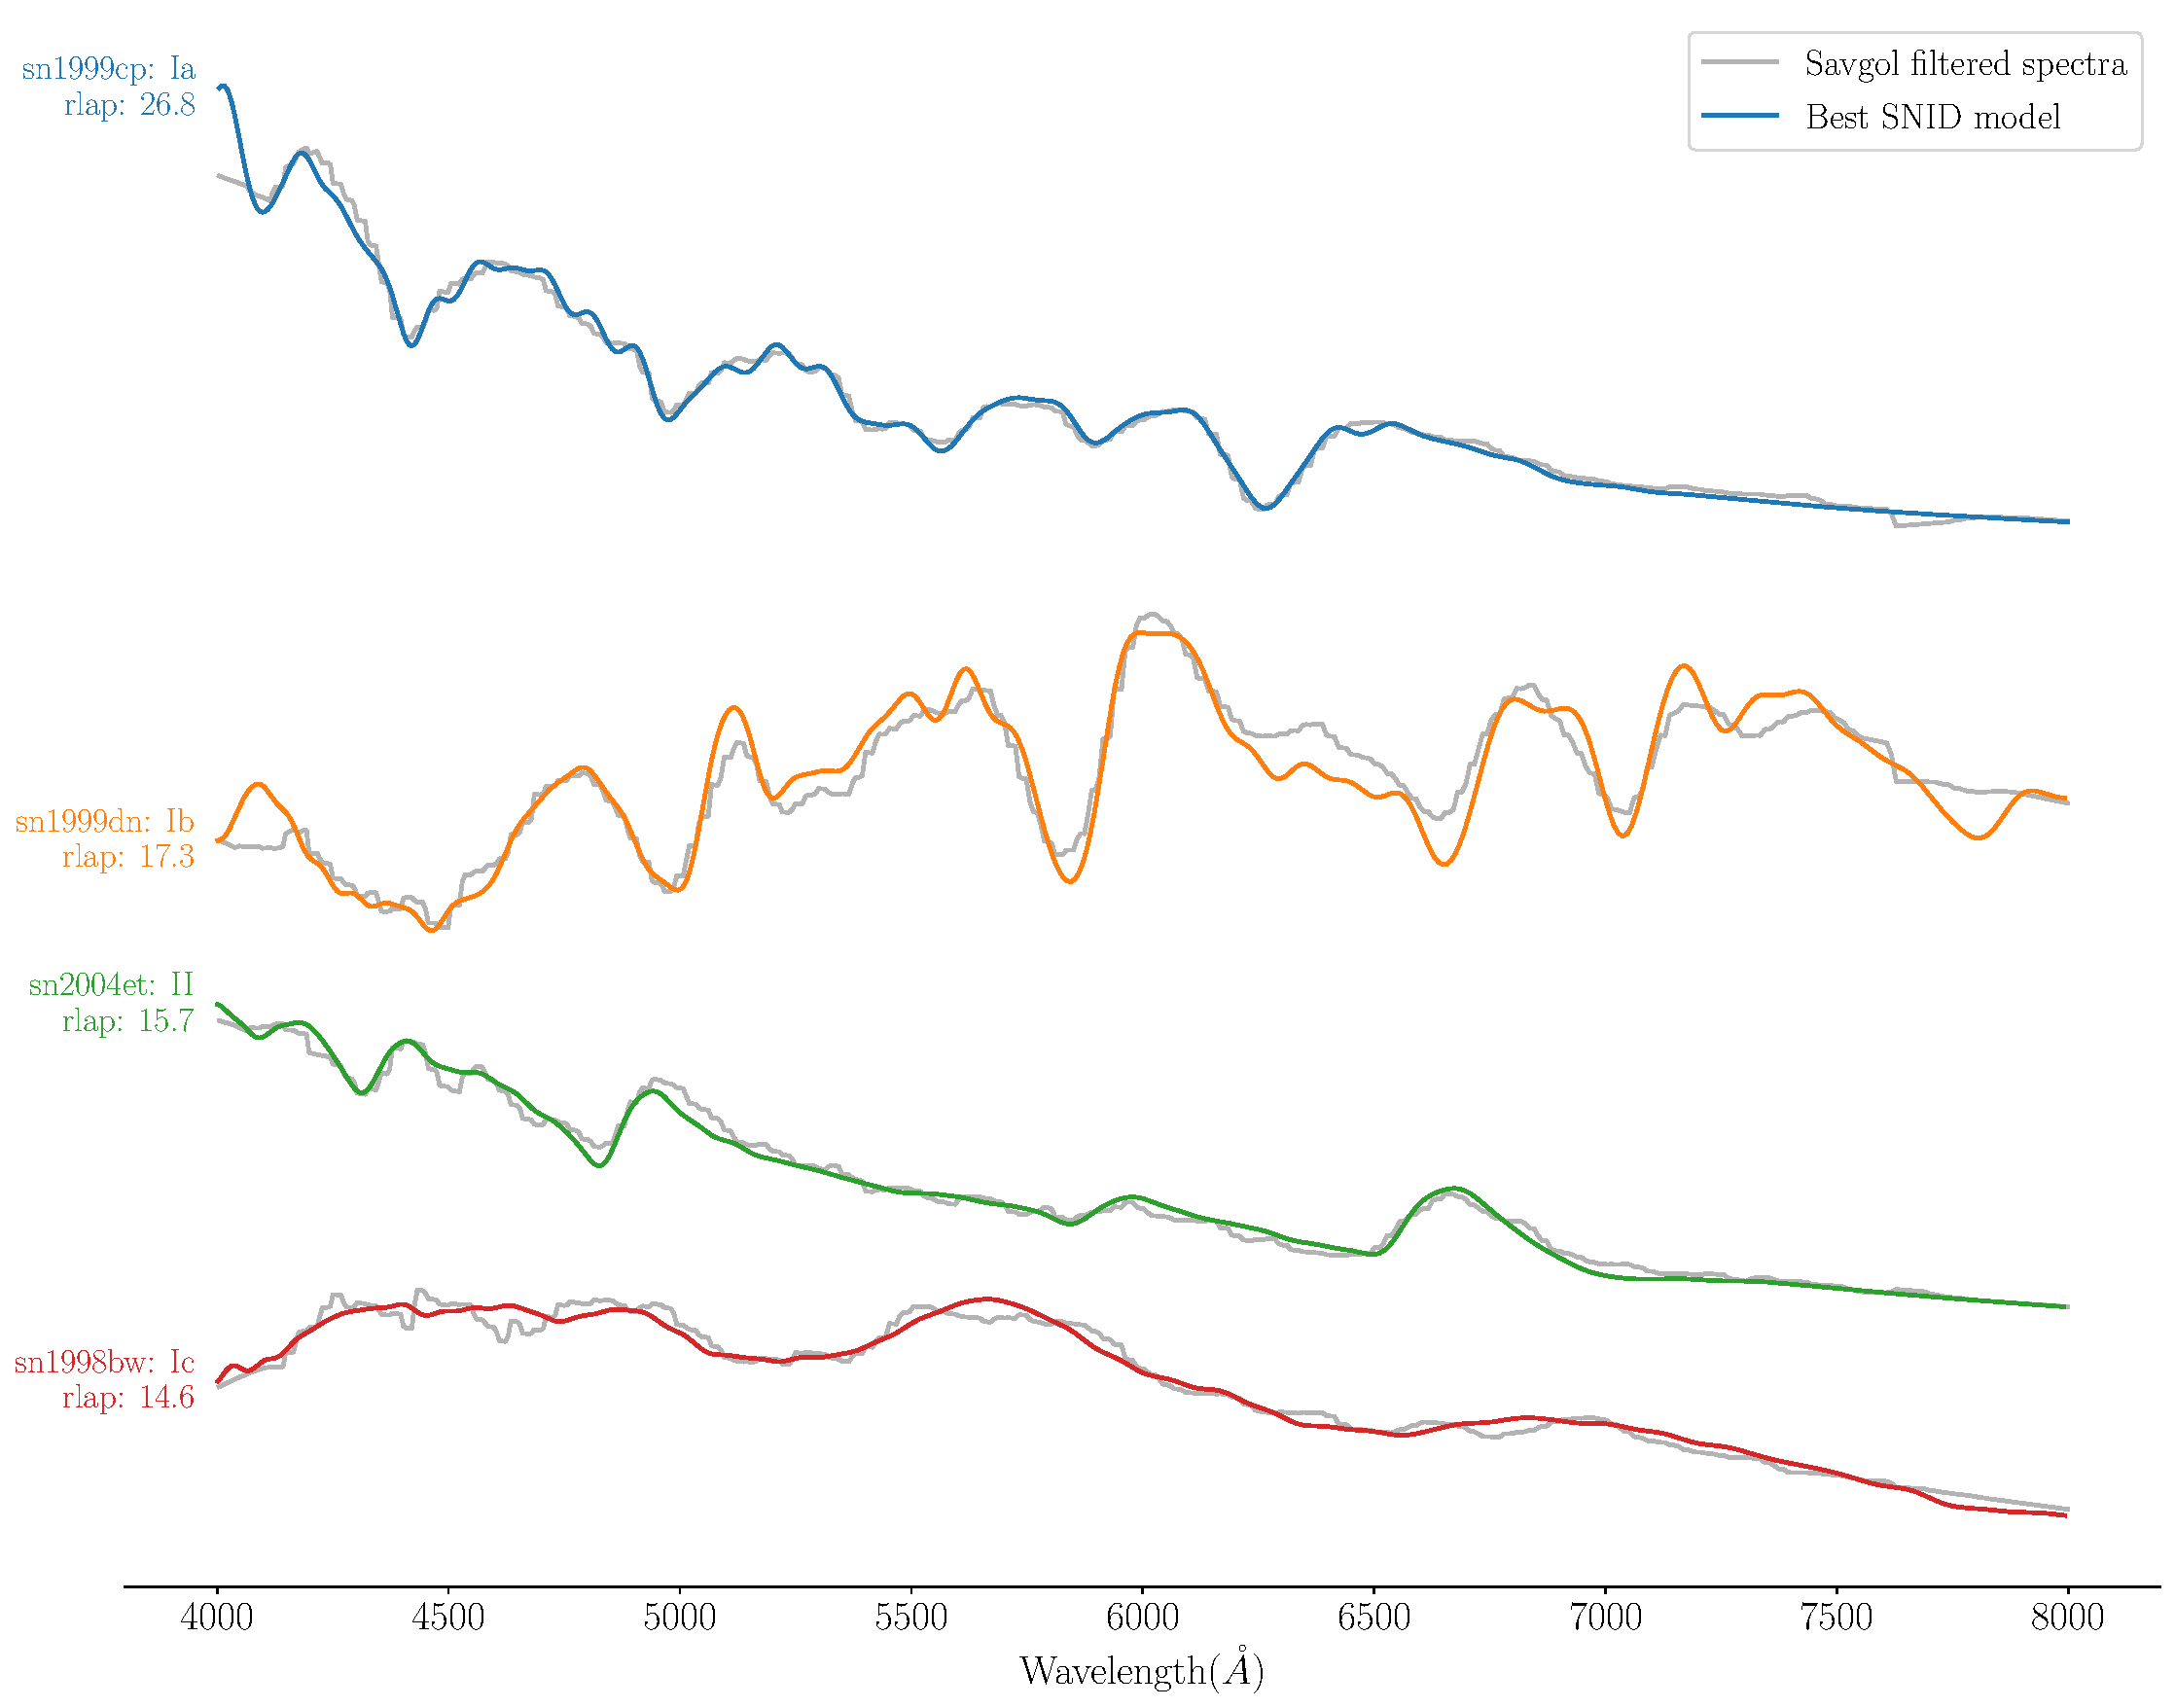
\includegraphics[width=0.99\textwidth]{../figures/08_simu/specsimueach.pdf}
  \caption[Exemple de spectre pour chaque type de supernova pour les
  simulations.]{Exemple de spectre pour chaque type de supernova pour
    les simulations. Nous y montrons en gris le spectre après
    lissage par un filtre de Savitzky-Golay, qui provient d'une
    observation de la SEDm. En couleur nous montrons le meilleur
  modèle de classification SNID et le r$lap$ associé, avec de haut en bas: une SNIa, une
  SNIb, une SNII, et une SNIc.}
  \label{fig:specsimueach}
\end{figure}

\subsection{Marginalisations et paramètres d'étude}
% \label{ssec:xxx}

\subsubsection{Types et phases}

Dans le but de représenter dans nos simulations les proportions
observées de chaque
type de supernova, nous utilisons les statistiques de la Data
Release 1 du groupe Bright Transient Survey de ZTF
\citep[BTS;][]{FremlingZTFspec2020}.
Nous choisissons ainsi de répartir dans nos simulations $80\%$ de SNIae,
$15\%$ de SNeII, $2.5\%$ de SNeIb et $2.5\%$ de SNeIc. Ces deux derniers
types sont habituellement regroupés, nous considèrerons donc par la
suite un groupe de $5\%$ de SNeIbc.

Nous choisissons également de 
procéder à une marginalisation des phases des spectres de SNIea, en se
basant sur les statistiques de la
DR1 du groupe SNeIa de ZTF \citep{DhawanZTFDR1}. Pour
les 70 spectres utilisés, nous déduisons la phase en comparant le
jour d'observation de la supernova dont est issu le spectre avec le pic
de luminosité ajusté par ZTF avec SALT2
\citep{Guysalt2005,Guysalt22007,Guy2010,Betoule2014} sur la courbe de
lumière.

La distribution de phase de notre échantillon s'étend de -15 à
+15 jours, avec une médiane à -2 jours. Nous pouvons ainsi sélectionner
aléatoirement les spectres de SNIa, sachant leur phase et suivant une
distribution équivalente à celle relevée dans \citep{DhawanZTFDR1}. Nous marginalisons nos simulations suivant
une distribution de phase gaussienne, centrée sur $-3$ jours et d'écart
type $4$ jours.

\subsubsection{Seeing}

Les supernovae étant des sources ponctuelles à ajouter dans nos cubes
de simulations, elles sont entièrement caractérisées par leur profil de
PSF.

Nous faisons l'hypothèse d'un profil connu a priori, et
utilisons le profil radial développé au chapitre~\ref{ch:irf} avec
l'étude des étoiles standards. Afin de représenter une distribution en
seeing similaire à celle observée par la SEDm, nous marginalisons nos
simulations sur le seeing en utilisant les
distributions conjointes des paramètres de forme de PSF ajustés des $2202$
étoiles standards extraites pour l'étude de la calibration en
flux (section~\ref{sec:validationpsf}).

Nous faisons donc la supposition que la distribution en seeing des
étoiles standards est représentative de celle des supernovae. Bien que
la contribution de l'optique du télescope soit indépendante
de l'objet observé, il faut noter que les étoiles standard le sont
habituellement avec une masse d'air comprise entre $1$ et
$1.2$. Nos simulations ayant une masse d'air comprise entre $1$ et $2$, cela implique potentiellement une sous-estimation que nous
n'avons pas caractérisé de la
distribution en seeing utilisée pour nos simulations.

\subsubsection{Distance supernova/centre galactique}\label{ssec:distancesimu}

\hypergal\ a été conçu pour répondre à la problématique de la
contamination par la galaxie hôte. Nous voulons donc explorer la
précision d'extraction de spectre des SNe et l'efficacité de
classification suivant la distance séparant la source ponctuelle du
cente galactique. Dans ces simulations nous ne nous intéressons pas aux
cas où la supernova est complètement isolée dans le champ de vue, ayant
déjà entrainé le pipeline avec les étoiles standards.

Nous utilisons une distribution uniforme comprise entre $0$ et $10$
spaxels de distance, ce qui correspond à un intervalle entre $0$ et
$\approx5\farcs6$. Cette distance seuil représente généralement environ $2$ à $3$ largeur à
mi-hauteur suivant le profil radial des sources ponctuelles, ce qui nous
semble suffisant pour explorer un large intervalle de séparation
angulaire jusqu'à la limite d'une isolation totale de la supernova.

Nous prenons également en compte que lors des observations réelles, les
supernovae sont habituellements situées vers le centre du MLA. Ainsi
afin d'éviter de simuler une cible dans un des coins du cube, nous
restreignons la localisation possible de la source ponctuelle dans un
disque de $12$ spaxels de rayon au centre du MLA. Pour les cas où la
galaxie est très excentrée et que nous simulons une source ponctuelle
proche du centre galactique, nous privilégions de la positionner dans le
quart de cercle en direction du centre du MLA. 

\subsubsection{Constraste}

Le dernier paramètre que nous utilisons pour explorer la robustesse
d'\hypergal\ correspond à l'intensité du flux de la supernova par
rapport à ce qui se situe à sa localisation: nous introduisons ainsi le
contraste $c_{r}$, défini dans la bande photométrique équivalente $ZTF_{r}$
afin de pouvoir plus aisément comparer les résultats des simulations
avec un cas réel d'observation, exprimé comme:
\begin{equation}
  \label{eq:contrast}
  c_{r} = \frac{S_{r}}{S_{r}+B_{r}}
\end{equation}
avec $S_{r}$ le signal de la supernova et $B_{r}$ le signal de tout ce qui se
situe en fond (ciel + galaxie).

Afin de déterminer la quantité $B_{r}$ qui contamine le signal de la
supernova, il faut prendre en compte le profil de PSF utilisé pour
simuler la source ponctuelle. En effet, si on suppose que la SN est
centrée (pour une longueur d'onde donnée) à la position ($x_{0}$,
$y_{0}$), alors le signal de fond à la même position aura un plus grand
impact de contamination que le fond à la position ($x_{0}+\d x_{0}$,
$y_{0}+\d y_{0}$).

Pour prendre cela en compte et plutôt que de considérer une ouverture fixe
autour de la localisation de la SN simulée pour définir $B_{r}$, nous
multiplions le cube de simulation sans la SN par un cube ne contenant
que le profil de PSF (normalisé avec un pic à $1$) à la localisation de
simulation de la SN.

Le contraste est ainsi défini dans l'intervalle $]0,1[$, $0$ impliquant
que la supernova n'existe pas, et $1$ qu'elle est infiniment plus
intense que le fond (ou que le fond est à zéro ce qui n'est pas notre
cas ici).

Nous pouvons également relier le contraste au rapport $R=\frac{S_{r}}{B_{r}}$:
\begin{equation}
  \label{eq:rapportSB}
  c_{r} = \frac{R}{1+R}
\end{equation}

Les simulations sont ainsi générées suivant une distribution uniforme du
contraste $c_{r}$ entre $0$ et $1$.

Nous pouvons également voir que le rapport signal sur bruit est
étroitement lié au contraste. En effet, en supposant que le signal dans
le cube est
entièrement caractérisée par une loi de Poisson, nous avons alors que:

\begin{equation}
  \label{eq:SNR}
  SNR_{r} \triangleq \frac{S_{r}}{\sqrt{\sigma_{S_{r}}^{2}+\sigma_{B_{r}}^{2}}}\approx
  \frac{S_{r}}{\sqrt{S_{r}+B_{r}}} = c_{r}\times\sqrt{S_{r}+B_{r}}
\end{equation}
avec $S_{r}$ et $B_{r}$ en unités de coups. Avec un raisonnement similaire nous
pouvons montrer que $SNR_{r}\approx R\times\sqrt{B_{r}}$.

En pratique, nous sommes en mesure de récupérer la quantité
$\sigma_{B}$, car présente dans le cube SEDm avec la galaxie hôte
isolée. Pour remonter au SNR, nous utilisons directement sa définition
en supposant que le bruit à ajouter dans le cube à cause du signal de la
supernova simulée est $\sigma_{S}^{2}=S$.

\subsection{Création des cubes de simulation}

Après avoir procéder à la marginalisation des proportions de chaque type
de supernova, de la phase des Ia et du seeing, nous générons un jeu de
$N\times m$ paramètres avec $N$ le nombre de simulations (5000), et $m$
les paramètres de la simulation:\\

\begin{itemize}[label=$\diamondsuit$]
  \itemsep0em
 \begin{samepage}
\item Cube de la galaxie hôte;
\item Spectre de supernova;
\item Paramètres de PSF décrivant la SN;
\item Distance entre la SN et le centre galactique;
\item  Contraste.
  \end{samepage}
\end{itemize}

Pour pouvoir ajouter le signal de la supernova simulée et surtout le
bruit associé, nous devons utiliser le cube SEDm en unité de flux
ADU et travailler dans ces unités avec le spectre de la SN.
Connaissant a priori la calibration en flux qui sera utilisé pour chacun des
cubes, nous appliquons une calibration inverse sur le spectre à simuler,
qui est initialement en unité de flux physique.

La création d'un cube de simulation sachant les $m$ paramètres se fait ensuite en plusieurs étapes:

\begin{minipage}{\textwidth}%
  \begin{enumerate}[(a)]
    \itemsep=0em
    \item \textbf{Détermination de la localisation ($x_{ref}$, $y_{ref}$) de la supernova} dans le cube
      à une longueur d'onde de référence ($\lambda_{ref}=6000$\AA):
      nous prenons aléatoirement une position sur le cercle centré sur
      la galaxie, avec un rayon égal à la distance simulée
      SN/galaxie. Nous prenons en compte les contraintes pour éviter les
      bords du cube expliquées dans la section~\ref{ssec:distancesimu};
      
  \item \textbf{Détermination du signal de fond $B$:} nous construisons un cube vide dans
    lequel nous plaçons le profil de PSF à la localisation et longueur
    d'onde fixée à l'étape
    précédente. La localisation est propagée pour toutes les tranches
    avec le modèle d'ADR, sachant les paramètres de masse d'air et
    d'angle parallactique, et le profil est normalisé à un pic égal à $1$ pour chaque
    longueur d'onde. Nous multiplions alors le cube de galaxie par
    celui-ci, le résultat étant un cube contenant uniquement le signal de fond $B$
    contaminant la SN.

  \item \textbf{Détermination du coefficient multiplicatif à appliquer sur le
    spectre de la supernova.} Nous déterminons grâce à l'étape précédente le fond contaminant $B_{r}$
    dans la bande équivalente $R$ de ZTF. Connaissant également le spectre de la
    supernova en ADU, nous en déduisons son signal $S'_{r}$ dans
    la bande $R$ avant adaptation au
    contraste souhaité. Enfin, connaissant $B_{r}$, $S'_{r}$ et $c_{r}$, nous
    appliquons le
    coefficient multiplicatif nécessaire sur l'ensemble du spectre de la
    SN (et donc sur $S'_{r}$) pour obtenir le constraste souhaité.

   \item \textbf{Ajout du bruit associé à la supernova.} Nous supposons que le
     flux ajouté de la supernova simulée est entièrement caractérisé
     par une loi de Poisson, et ajoutons donc au cube SEDm pour chaque
     spaxel de chaque tranche une variance telle que $\sigma_{S,\lambda,spx}^{2}=S_{\lambda,spx}$.

   \item \textbf{Détermination du SNR.} Le SNR n'est pas un paramètre de
     nos simulations, mais nous pouvons le récupérer et le stocker connaissant
     $B_{r}$, $S_{r}$, $\sigma_{B_{r}}$ et  $\sigma_{S_{r}}$.

   \item \textbf{Construction du cube de simulation}. Tous les
     ingrédients sont réunis pour la construction du cube: le spectre de
     la supernova, sa position chromatique, son profil de PSF
     chromatique et le coefficient multiplicatif pour avoir le contraste désiré.
  \end{enumerate}
\end{minipage}\\


Nous procédons ainsi à la générations des $5000$ cubes de
simulations. Dans la Figure~\ref{fig:examplesimu} nous illustrons
quelques exemples de ces cubes pour différentes valeurs de contraste,
distance, type de SN et SNR.
\begin{figure}[ht]
  \centering
  \makebox[\textwidth][c]{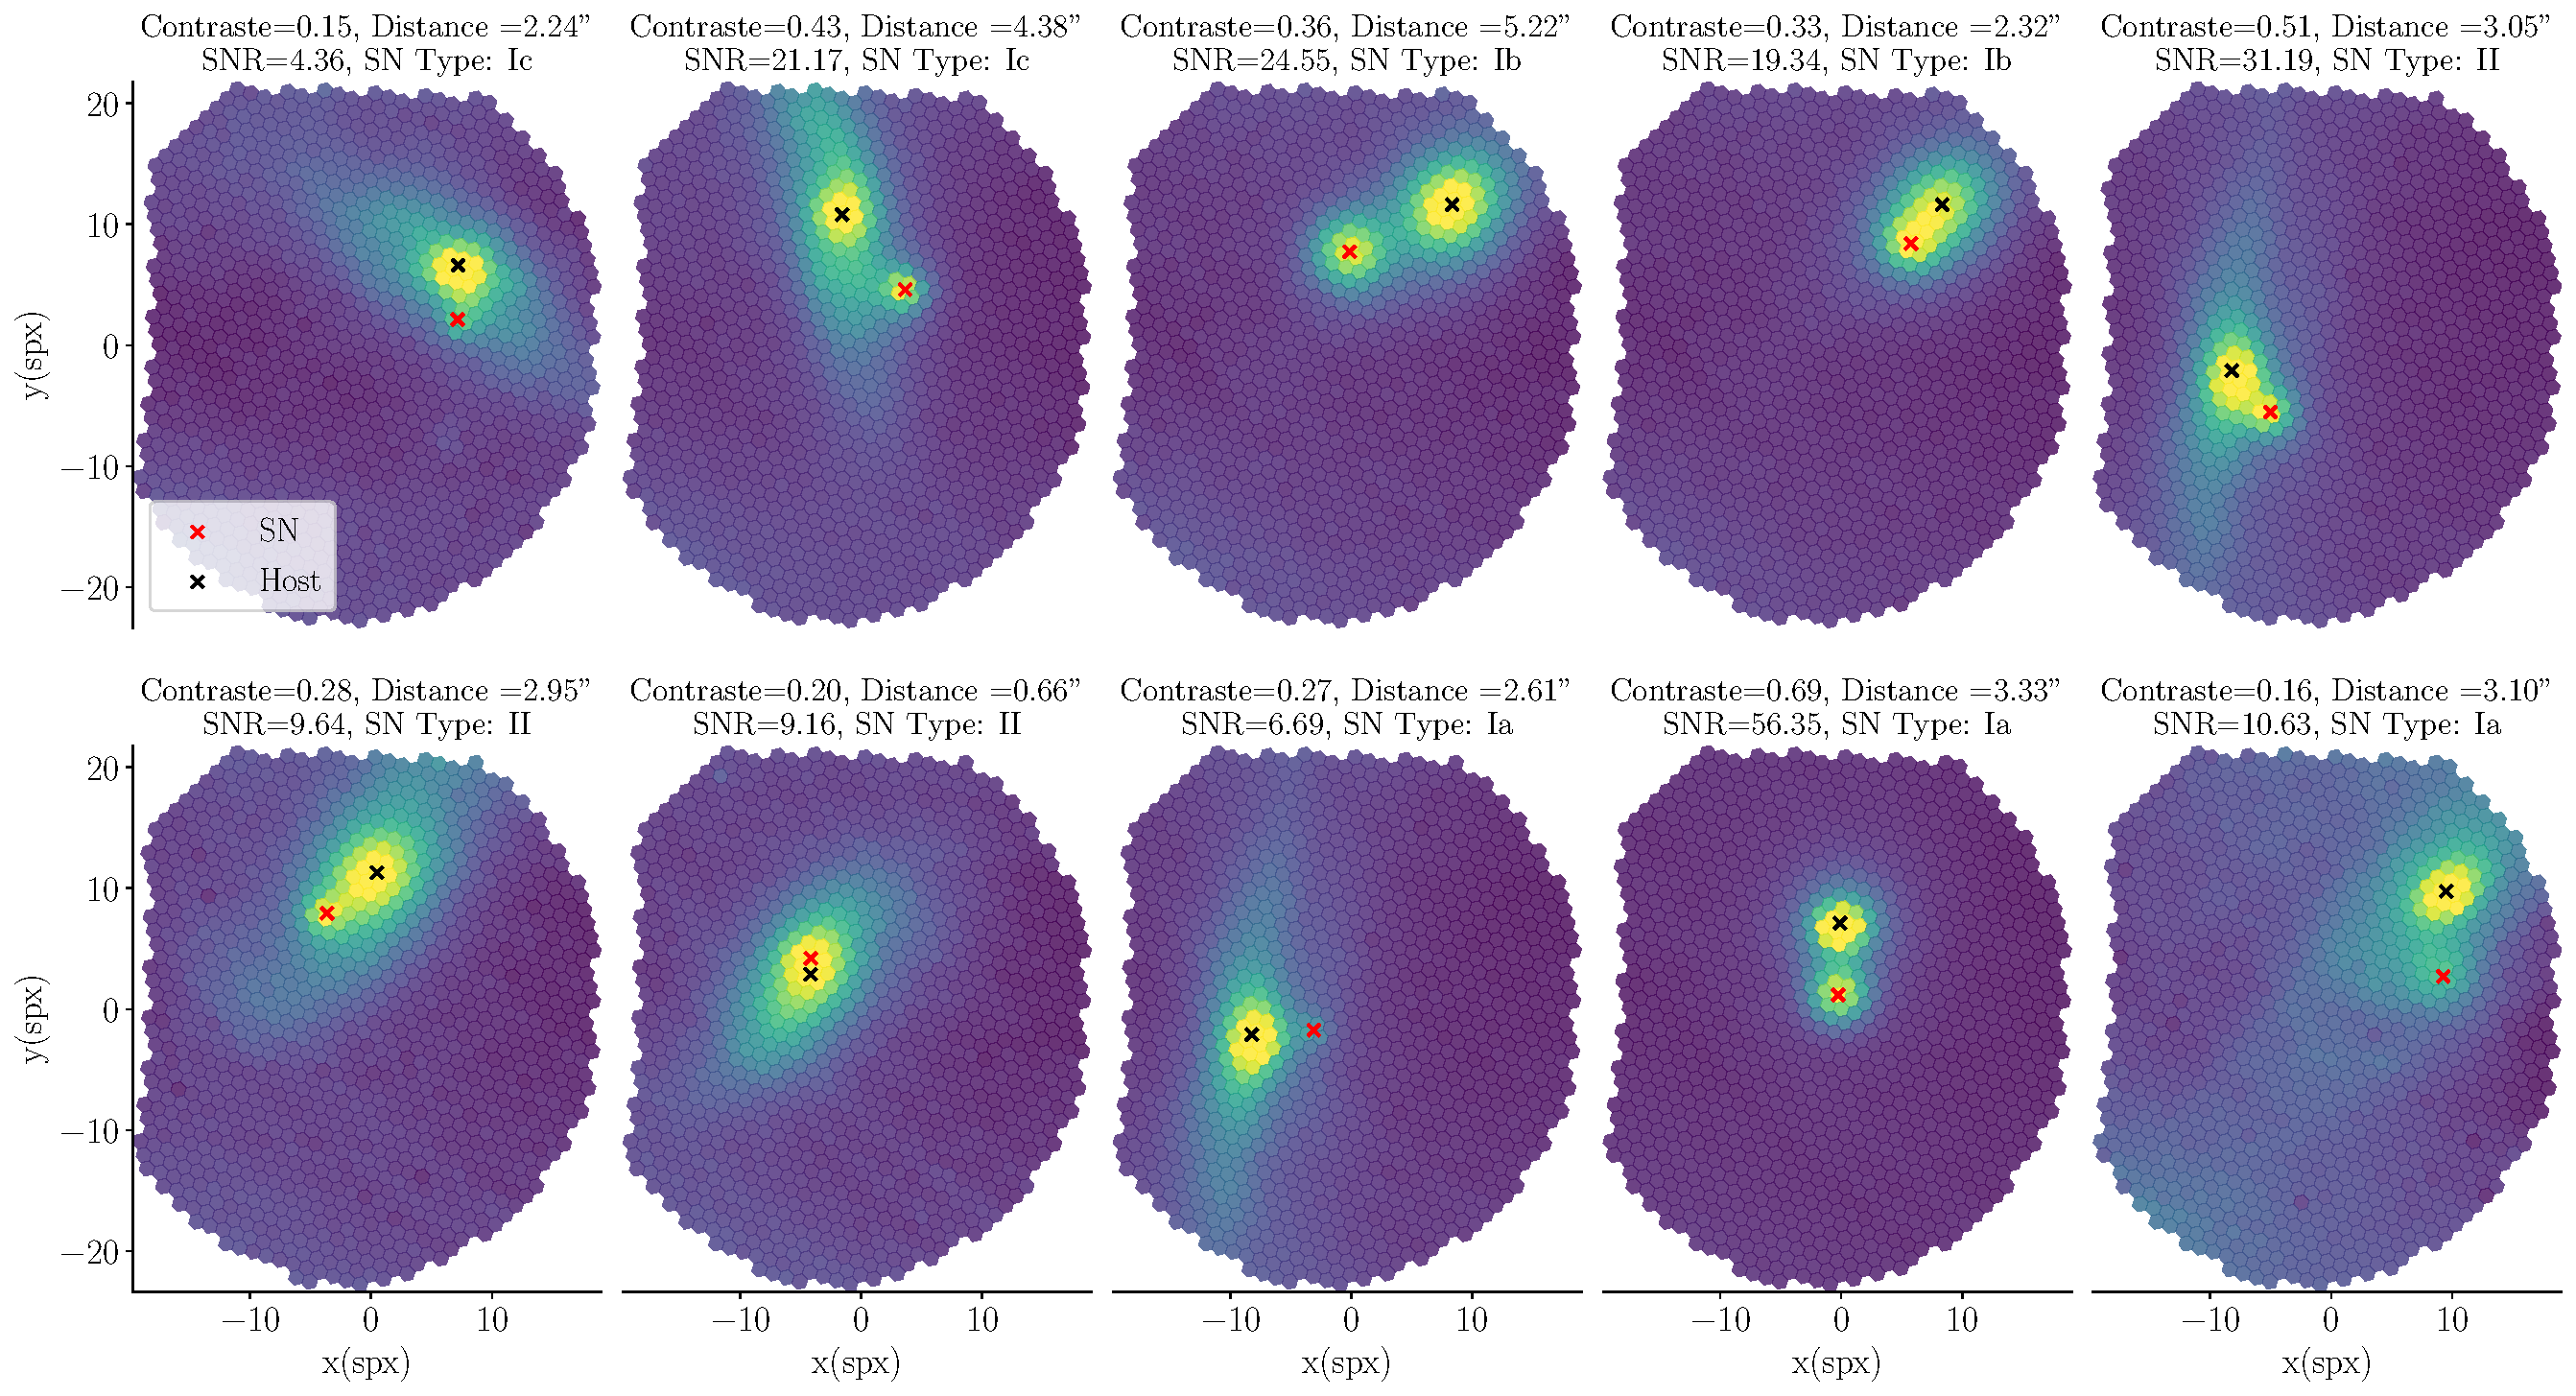
\includegraphics[width=1.15\textwidth]{../figures/08_simu/examplesimu.pdf}}%
  \caption[Examples de cubes de simulation.]{Examples de cubes de
    simulation pour différentes valeurs de contraste, distance, type de
    SN et SNR.}
  \label{fig:examplesimu}
\end{figure}

\section{Résultats et précision}\label{sec:simuresult}

Après avoir généré nos cubes de simulation, nous avons fait tourner
\hypergal\ suivant 2 méthodes: la première avec une modélisation de
scène comprenant toutes les composantes comme détaillée au chapitre
précédent. Et une deuxième fois avec la même méthode d'extraction que le
pipeline d'origine \pysedm, sans modélisation de la galaxie hôte.

Nous n'avons pas utilisé directement le pipeline \pysedm\ car les modèles
de PSF et de fond sont différents de celui d'\hypergal, ce qui n'aurait
pas permis une comparaison robuste. La méthode d'extraction est cela dit
identique, suivant le procédé détaillé dans \citet{pysedm} et la section~\ref{ssec:sourceextractpysedm}.
Les seules différences avec la modélisation de scène complète étant
l'absence de modèle de galaxie, et le fait que l'on ne considère qu'un
disque de $10$ spaxels de rayon autour de la position de la supernova
pour son extraction.

En plus d'une étude de la robustesse absolue d'\hypergal, cette
confrontation nous permet d'avoir également une idée de l'amélioration
apportée avec ce nouvel outil d'extraction de spectre.

Nous dénominerons dans la suite du manuscrit l'indice $_{HG}$ pour la
méthode de modélisation de scène \hypergal, et $RMS_{PS}$ pour la méthode
d'extraction de source ponctuelle basique.

Dans cette section nous allons étudier 3 informations pour chacune des 2
méthodes:

\begin{itemize}[label=$\diamondsuit$]
  \itemsep0em
 \begin{samepage}
\item \textbf{La précision spectrophotométrique}, c'est à dire une
  comparaison brute du spectre de simulation et du spectre extrait;
\item \textbf{La précision après correction du continuum}, à l'instar de
  la méthode de pré-traitement utilisé dans \pkg{SNID}
  (section~\ref{sec:snid}). La SEDm ayant été conçu pour la
  classification de spectres, ce qui nous importe est la
  capacité d'\hypergal\ à extraire les informations spectrales
  permettant cette classification, c'est à dire la structure du spectre
  traduisant les caractéristiques de tel ou tel type.
\item \textbf{L'efficacité de classification}. Pour cela nous
  utiliserons le même classifieur utilisé par ZTF, \pkg{SNID}, et nous
  comparerons la classification du spectre extrait avec celui connu a priori.
  \end{samepage}
\end{itemize}

\subsection{Précision spectrophotométrique}
%\label{ssec:xxx}


\begin{figure}[ht]
  \centering
  \makebox[\textwidth][c]{\includegraphics[width=1.\textwidth]{../figures/08_simu/simu_rms_snr_spectrophoto.png}}%
  \caption[]{}
  \label{fig:simu_rms_snr_spectrophoto}
\end{figure}

\begin{figure}[ht]
  \centering
  \makebox[\textwidth][c]{\includegraphics[width=1.\textwidth]{../figures/08_simu/simu_rms_dist_spectrophoto.png}}%
  \caption[]{}
  \label{fig:simu_rms_dist_spectrophoto}
\end{figure}


\subsection{Précision avec correction de continuum}
% \label{ssec:xxx}

\begin{figure}[ht]
  \centering
  \makebox[\textwidth][c]{\includegraphics[width=1.\textwidth]{../figures/08_simu/simu_rms_snr_continuum_divided.png}}%
  \caption[]{}
  \label{fig:simu_rms_snr_continuum_divided}
\end{figure}

\begin{figure}[ht]
  \centering
  \makebox[\textwidth][c]{\includegraphics[width=1.\textwidth]{../figures/08_simu/simu_rms_dist_continuum_divided.png}}%
  \caption[]{}
  \label{fig:simu_rms_dist_continuum_divided}
\end{figure}

\subsection{Efficacité de classification}
% \label{ssec:xxx}


\begin{figure}[ht]
  \centering
  \makebox[\textwidth][c]{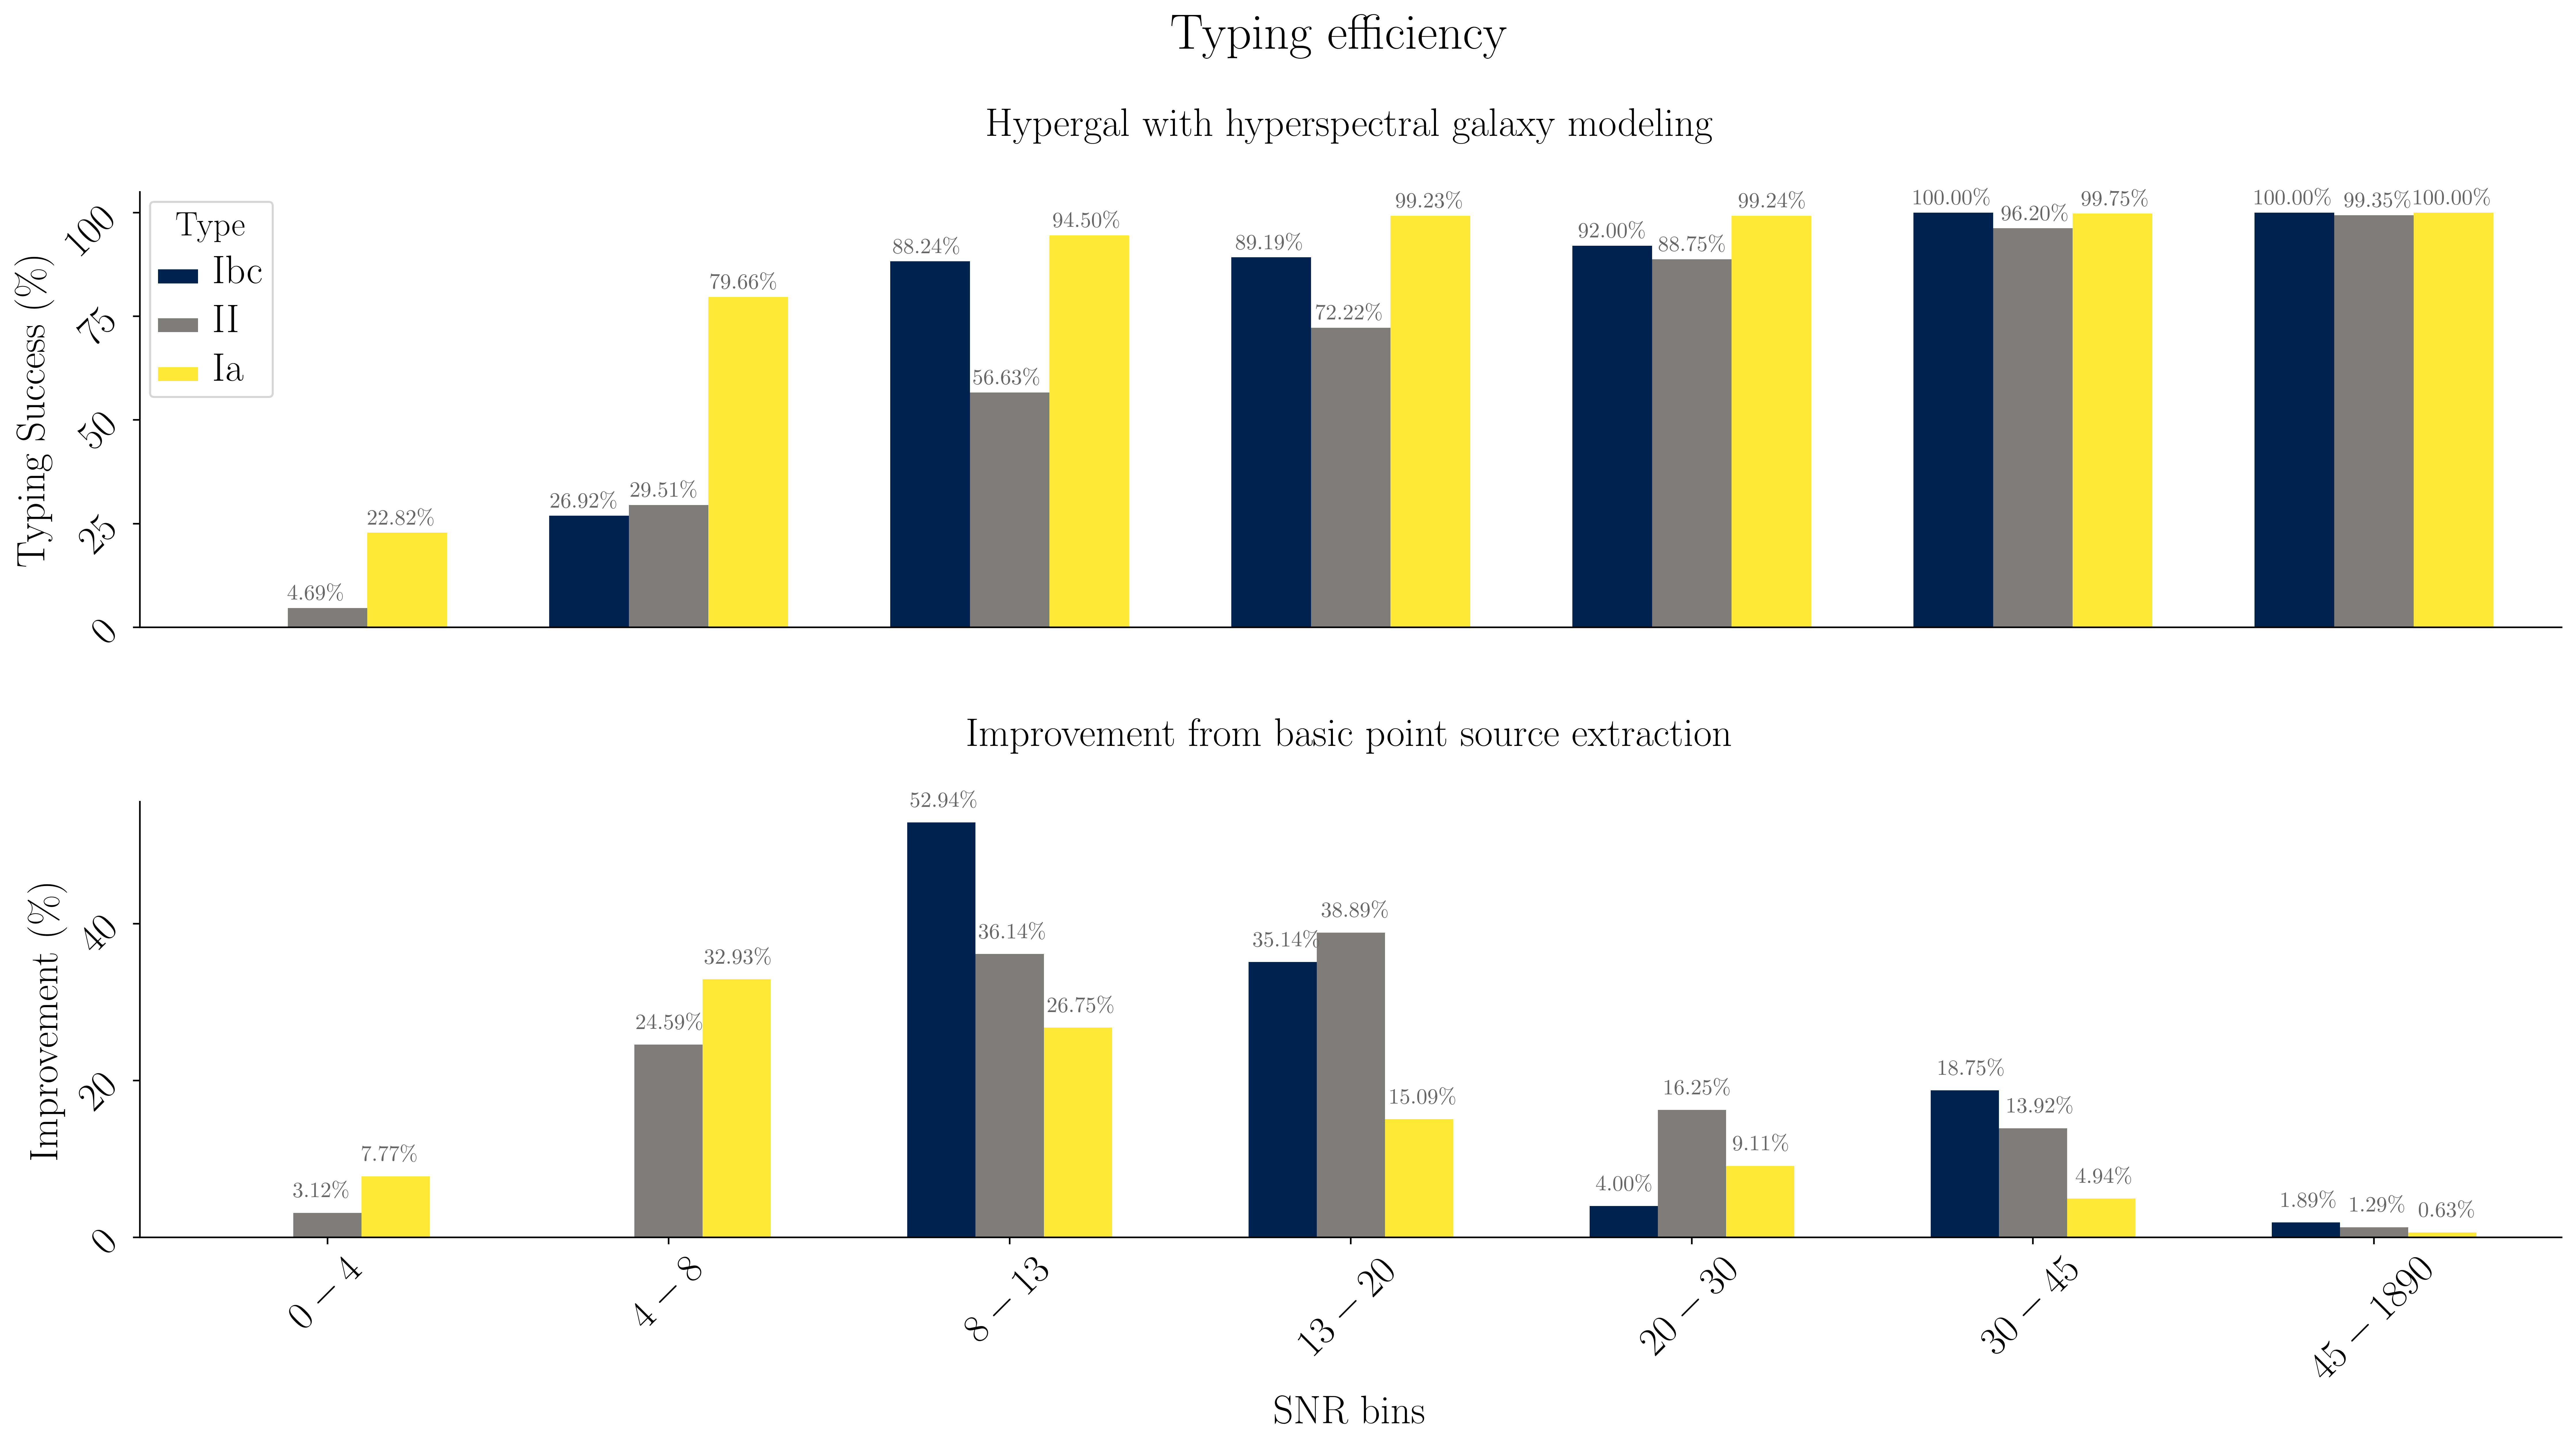
\includegraphics[width=1.2\textwidth]{../figures/08_simu/typingimprove_snr.png}}%
  \caption[]{}
  \label{fig:typingimprove_snr}
\end{figure}

\bibliographystyle{../main/aa_url2}
\bibliography{99_references}
\end{document}

%%% Local Variables:
%%% mode: latex
%%% TeX-master: t
%%% End:
